\section{Desarrollo}

\section{Ejercicio 2}
La solución óptima para los coeficientes del ecualizador debe cumplir con la siguiente expresión:

\begin{equation}
	\textbf{R}_Y \textbf{w}_o = \textbf{R}_{YX}
\end{equation}

$\textbf{R}_Y$ es la matriz de Toeplitz de la autocorrelación de $Y$. Luego, la matriz $\textbf{R}_{YX}$ es: 

\[
\mathbf{R}_{YX} = \mathbb{E}
\begin{bmatrix}
	y(n) x(n) \\
	y(n-1) x(n) \\
	\vdots \\
	y(n - m + 1) x(n)
\end{bmatrix}
=
\begin{bmatrix}
	R_{yx}(0) \\
	R_{yx}(1) \\
	\vdots \\
	R_{yx}(m-1)
\end{bmatrix}
=
\begin{bmatrix}
	h(0) \\
	h(-1) \\
	\vdots \\
	h(-m+1)
\end{bmatrix}
=
\begin{bmatrix}
	h(0) \\
	0 \\
	\vdots \\
	0
\end{bmatrix}
\]

Finalmente $\textbf{w}_o$ es un vector que se obtiene de operar de la siguiente manera con las matrices previamente mencionadas.

\begin{equation}
	\textbf{w}_o = \textbf{R}_Y^{-1} \cdot \textbf{R}_{YX}
\end{equation}

\section{Ejercicio 3}

Como se demuestra en la (REFERENCIAR seccion 1), las matrices con las que se calculan los coeficientes óptimos para el equalizador dependen solamente de los coeficientes del modelo del canal. Luego se simuló la secuencia $X(n)$ y en base a ella se calcularon las secuencias $Y(n)$ y $Z(n)$ usando la funcion \verb*|filter| con $\textbf{h}$ y $\textbf{w}_o$. La figura~\ref{fig:ej3_x} muestra como la autocorrelación de $X(n)$ resulta en algo similar a una delta en el origen y la PSD resulta ruidosa, pero relativamente constante. En la figura~\ref{fig:ej3_y} se observan los atributos de la secuencia $Y(n)$, es decir como termina $X(n)$ una vez que atraviesa el canal. Como era de esperar, la señal se distorsiona considerablemente, ya que tanto la secuencia, como su autocorrelación y PSD difieren mucho de $X(n)$. Por último, La figura~\ref{fig:ej3_z} muestra una secuencia casi idéntica a la de entrada, demostrando que el equalizador funcionó correctamente.

En la figura~\ref{fig:ej3_coef} se muestra una comparación de los coeficientes del modelo del canal y los coeficientes del equalizador obtenidos. 

\begin{figure}[h]
	\centering
	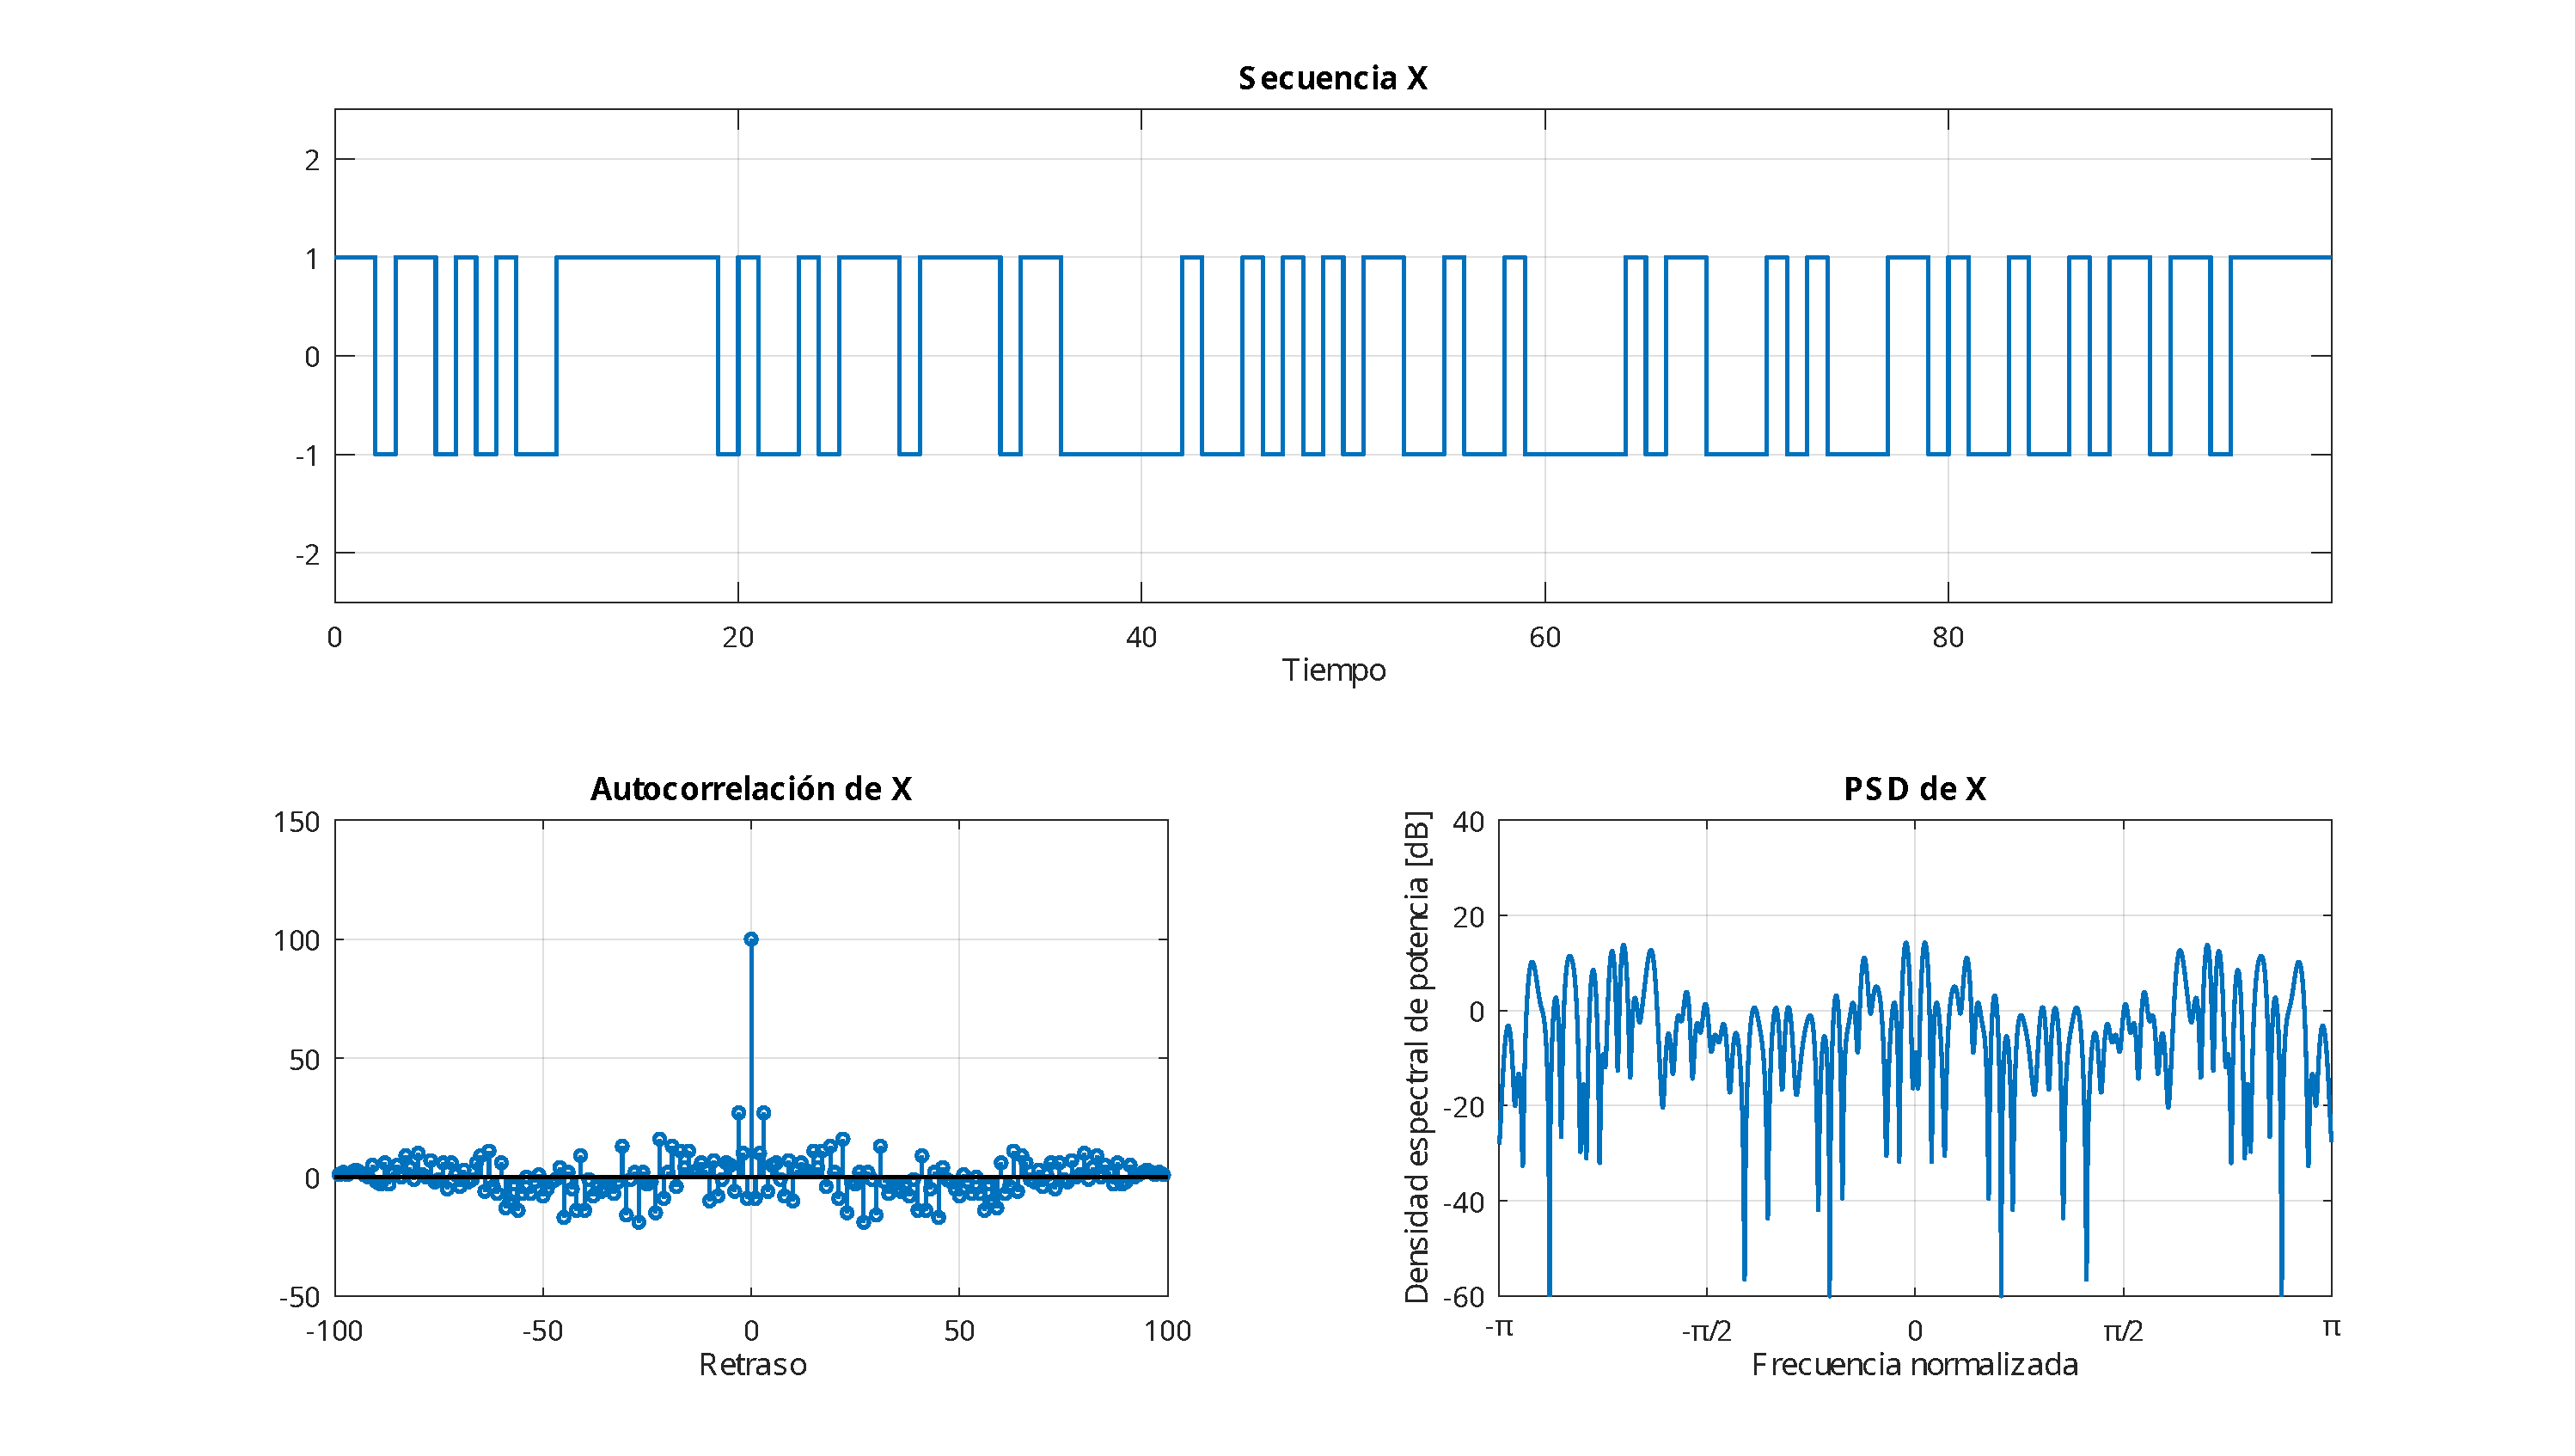
\includegraphics[width=1\linewidth]{img/ej3_x.pdf}
	\caption{Secuencia, autocorrelación y PSD de $X(n)$.}
	\label{fig:ej3_x}
\end{figure}

\begin{figure}[h]
	\centering
	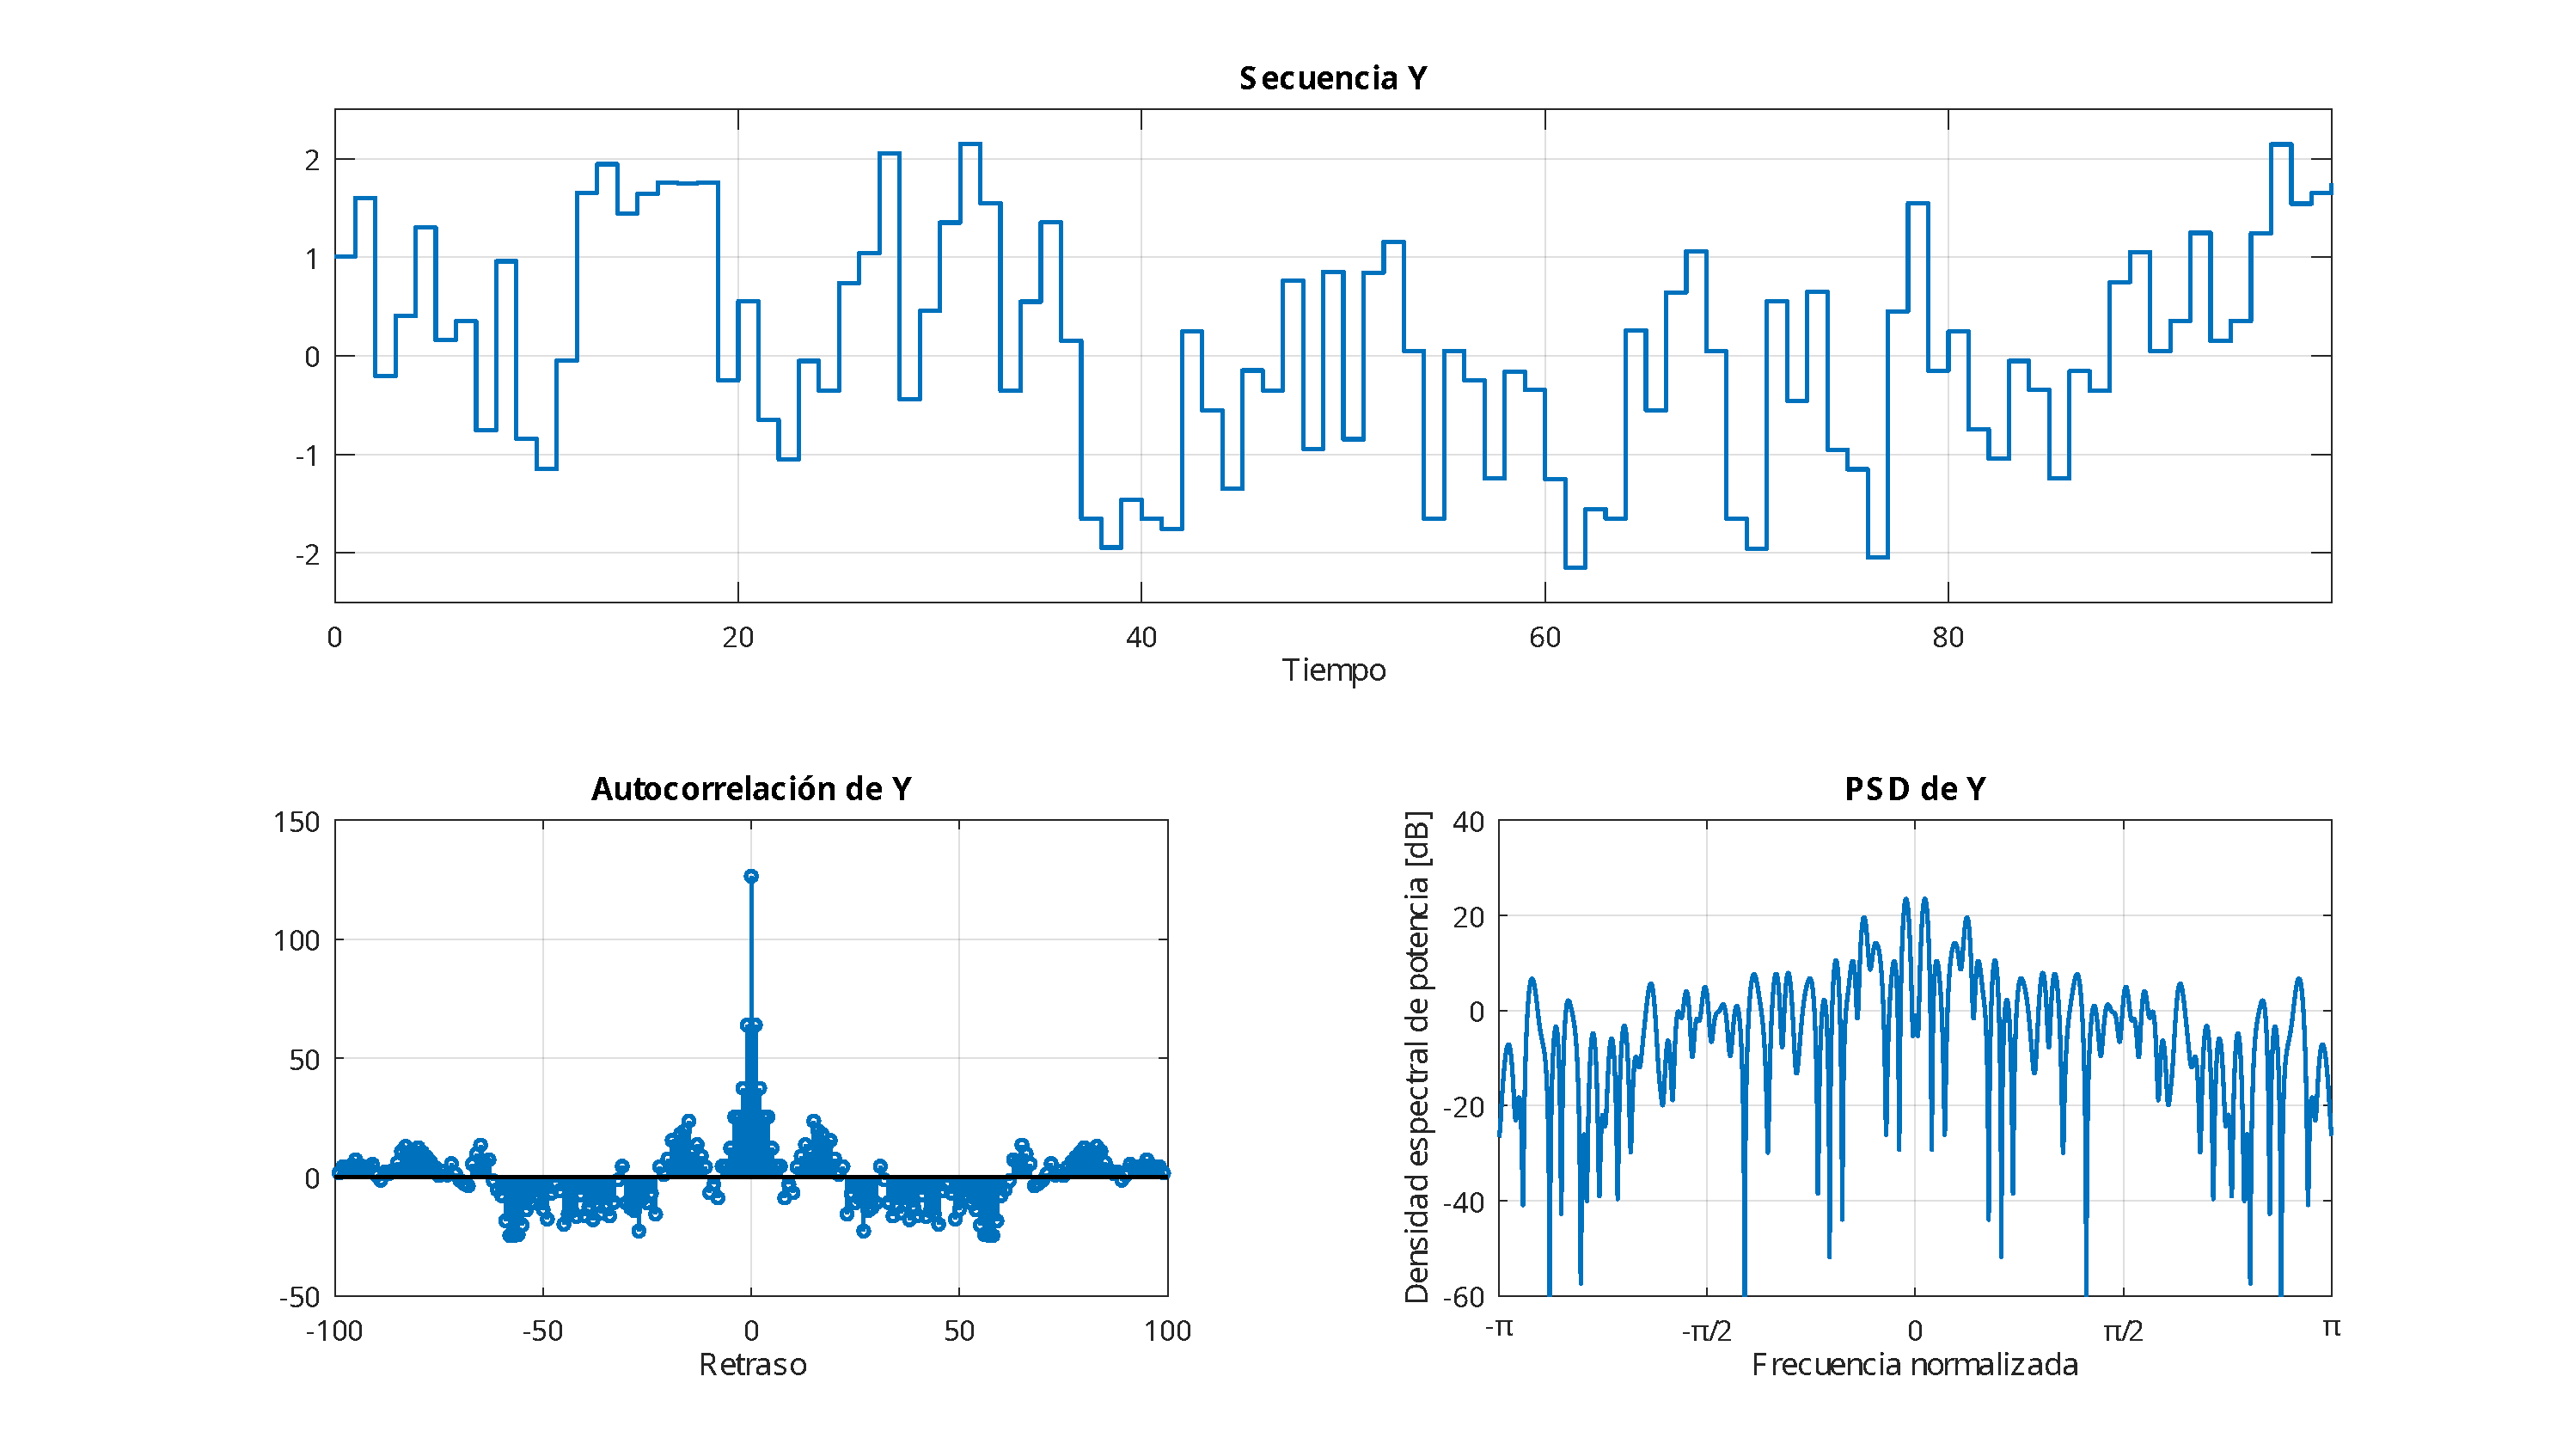
\includegraphics[width=1\linewidth]{img/ej3_y.pdf}
	\caption{Secuencia, autocorrelación y PSD de $Y(n)$.}
	\label{fig:ej3_y}
\end{figure}

\begin{figure}[h]
	\centering
	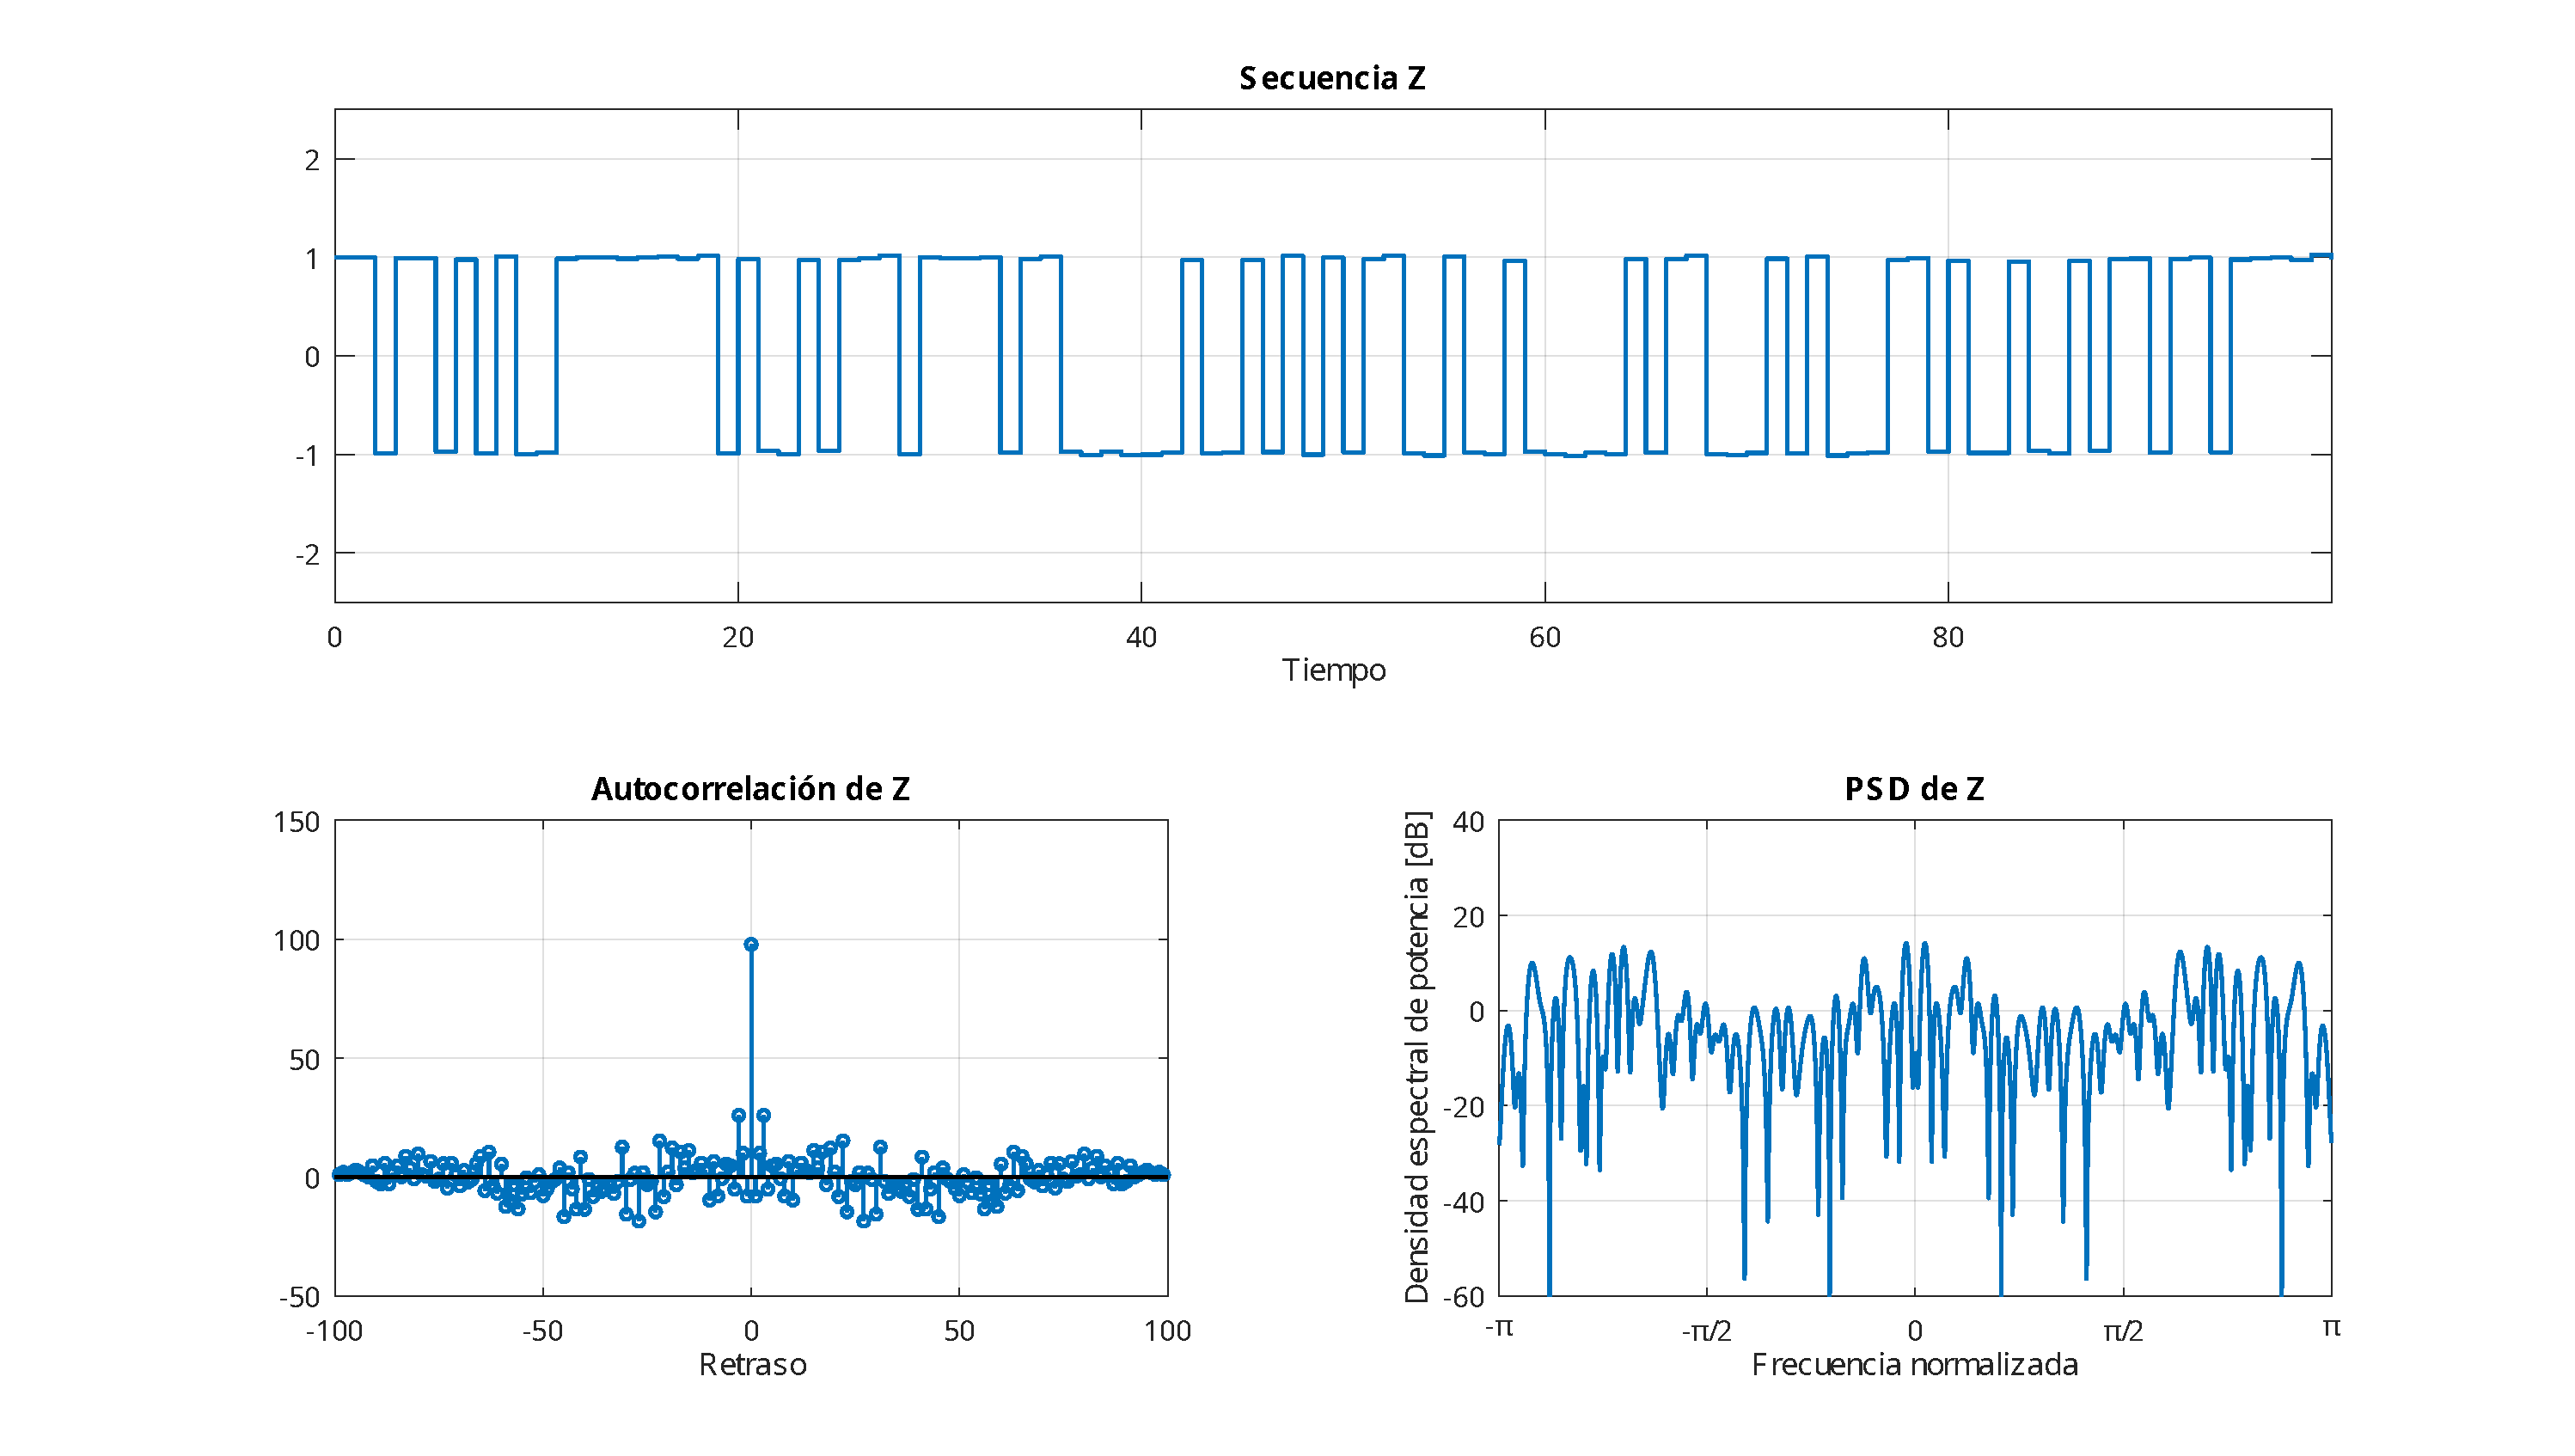
\includegraphics[width=1\linewidth]{img/ej3_z.pdf}
	\caption{Secuencia, autocorrelación y PSD de $Z(n)$.}
	\label{fig:ej3_z}
\end{figure}

\begin{figure}[h]
	\centering
	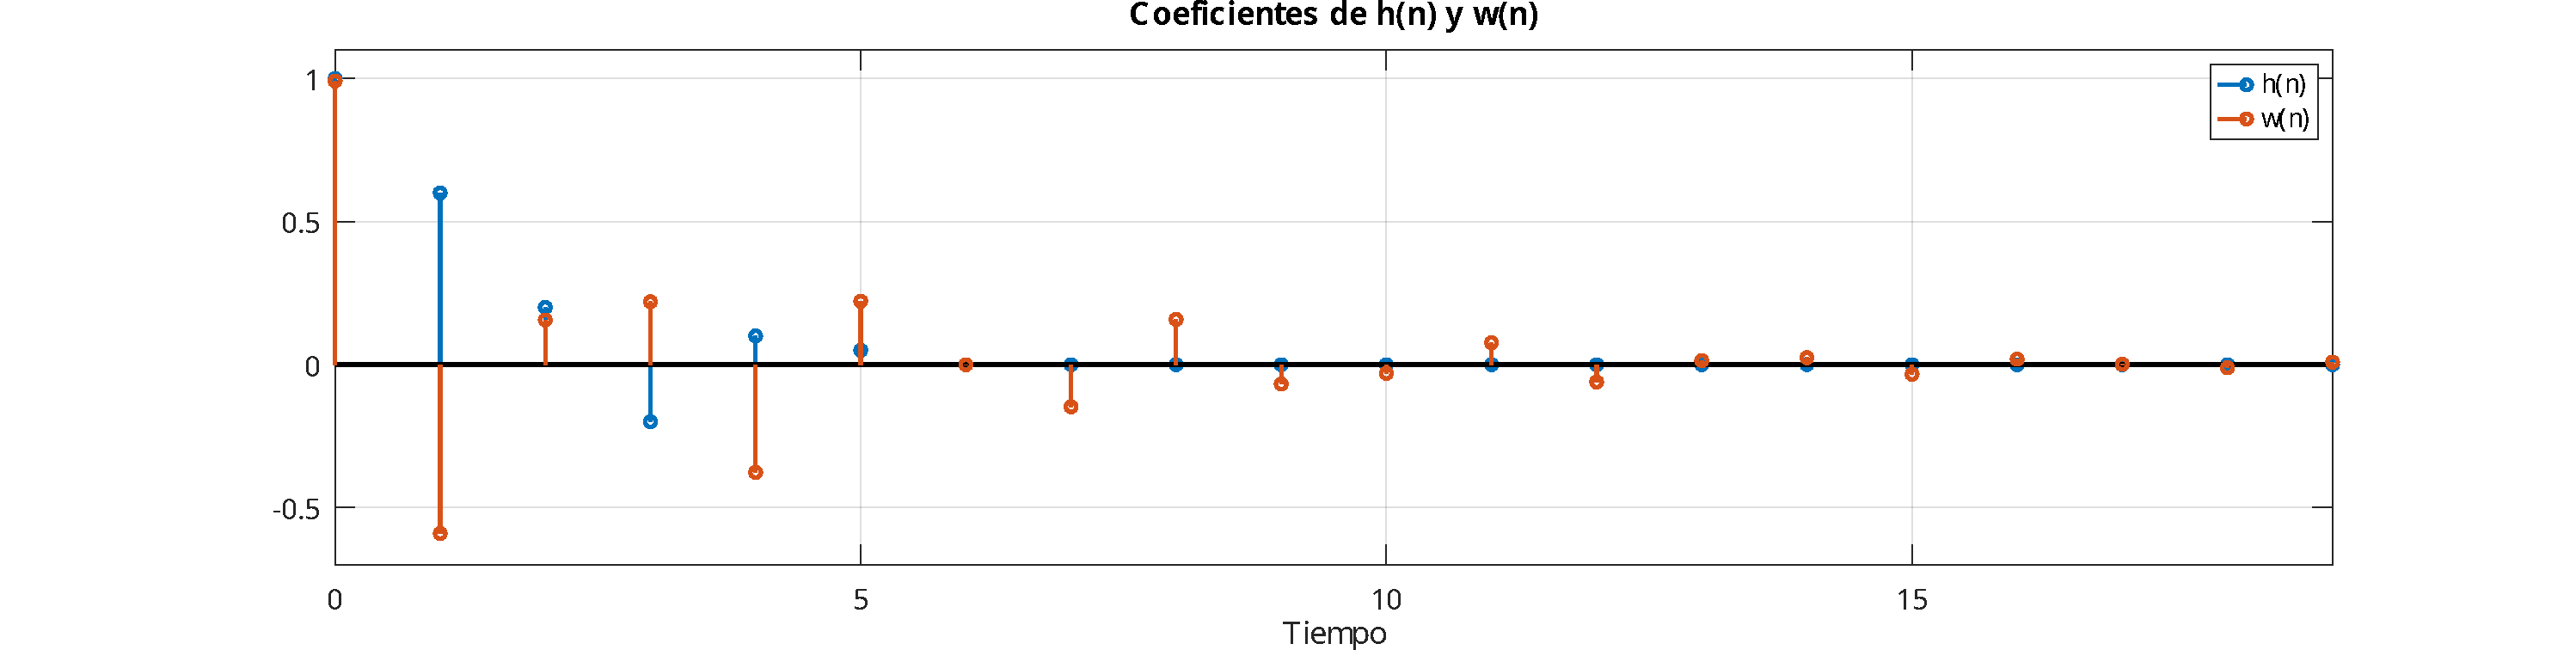
\includegraphics[width=1\linewidth]{img/ej3_coef.pdf}
	\caption{Comparación de $h$ y $w$.}
	\label{fig:ej3_coef}
\end{figure}